% !TeX encoding = UTF-8
% !TeX program = pdflatex
% !BIB program = biber

\documentclass[
        english,biblatex
    ]{lni}

\addbibresource{my-paper.bib}


% Standard packages
\usepackage{graphicx}
\usepackage{longtable}
\usepackage{booktabs}
\usepackage{array}
\usepackage{multirow}
\usepackage{wrapfig}
\usepackage{float}
\usepackage{colortbl}
\usepackage{pdflscape}
\usepackage{tabularx}
\usepackage{threeparttable}
\usepackage{threeparttablex}
\usepackage[normalem]{ulem}
\usepackage{makecell}
\usepackage{multicol}


\usepackage{framed} % Needed for code blocks


% solve \tightlist error
\providecommand{\tightlist}{%
    \setlength{\itemsep}{0pt}\setlength{\parskip}{0pt}}

% solve \pandocbounded error
\providecommand{\pandocbounded}[1]{#1}



\begin{document}

% Title
        \title[]{Comparing Research Software Engineering and Data
Science Competences}
    
    
    %\usepackage{hyperref}

    


\author[1]{Julian Dehne}{julian.dehne@gi.de}{0000-0001-9265-9619}
\author[2]{Jan Philipp Thiele}{jan-philipp.thiele@tu-braunschweig.de}{0000-0002-8901-6660}
\author[3]{Jeremy Cohen}{jeremy.cohen@imperial.ac.uk}{0000-0003-4312-2537}
\author[4]{Katrin Schöning-Stierand}{\href{mailto:katrin.schoening-stierand@uni-hamburg.de}{katrin.schoening-stierand@uni-hamburg.de}}{0000-0003-3248-8023}
\author[5]{Florian Goth}{\href{mailto:Florian.Goth@uni-wuerzburg.de}{Florian.Goth@uni-uerzburg.de}}{0000-0003-2707-4790}
\author[6]{Jan Linxweiler}{\href{mailto:j.linxweiler@tu-braunschweig.de}{j.linxweiler@tu-braunschweig.de}}{0000-0002-2755-5087}
\author[7]{Anna-Lena Lamprecht}{\href{mailto:anna-lena.lamprecht@uni-potsdam.de}{anna-lena.lamprecht@uni-potsdam.de}}{0000-0003-1953-5606}

\affil[1]{Gesellschaft für Informatik\\Bildung und Gesellschaft\\
Weydingerstraße 14-16\\10178 Berlin\\Deutschland}
\affil[2]{TU Braunschweig\\Universitätsbibliothek\\
Universitätspl. 1, 38106 Braunschweig\\Deutschland}
\affil[3]{University 3\\Department\\Address\\Country}
\affil[4]{Universität Hamburg\\Hub of Computing and Data Science\\Albert-Einstein-Ring 8\\22761 Hamburg\\Deutschland}
\affil[5]{Universität Würzburg\\Institut für theoretische Physik 1\\Am Hubland\\97070 Würzburg\\Deutschland}
\affil[6]{TU Braunschweig\\Universitätsbibliothek\\
Universitätspl. 1, 38106 Braunschweig\\Deutschland}
\affil[7]{Universität Potsdam\\Chair of Software Engineering\\An der Bahn 2\\14476 Potsdam\\Deutschland}


    \maketitle

% Abstract
        \begin{abstract}
        Research Software Engineers (RSEs) and Data Scientists (DSs)
        have overlapping yet distinct roles within the landscape of
        digitally skilled professionals. Both roles are highly
        software-focused and operate across a wide range of research
        domains, yet their communities and competency frameworks have
        evolved independently. This paper explores the intersections and
        distinctions between RSE and DS competencies, particularly as
        they relate to different phases of the research cycle.
    \end{abstract}
    
% Keywords
        \begin{keywords}
        Research Software Engineering \and Data Science \and Competences
    \end{keywords}
    
% Body
    \section{Introduction}\label{introduction}

    Computers and software have become vital elements of the research
    process across almost all domains. They enable researchers to
    collect and process ever-increasing amounts of data, simulate a wide
    range of phenomena on previously unexplored scales, and discover
    previously inconceivably complex structures in nature and societies
    via machine learning (ML). This importance of computation and
    digitally-aided data analysis in research means that digital skills
    are now required by researchers at all career levels. However, as
    there is a much wider range of digital skills required to support
    the modern research lifecycle than an individual researcher can
    master to perfection, there is increasing demand for people in
    specialist technical roles who can interface between researchers and
    their digital tools and processes. These technical professionals
    (increasingly becoming known within the UK research community as
    ``digital Research Technical Professionals'' -- dRTPs), provide
    targeted help, support and specialist technical expertise to
    researchers. Below we introduce some of the technical roles that
    have emerged in the research landscape over recent years (roughly in
    the order in which the terms started appearing).

    \begin{itemize}
    \item
      \textbf{Research Data Managers} (also know as Data Stewards)
      support the handling of data throughout the research data
      life-cycle including data acquisition, processing, storage and
      publication. The efficiency, validity and recognition of research
      in many domains today hinges on the quality, availability and
      reproducibility of data and data-transforming methods. Research
      Data Management (RDM) therefore has become a cross-cutting field
      with a large number of sub-topics that range from legal themes,
      e.g.~licenses, data usage agreements and data protection laws over
      technical themes related to the organization, storage, transport,
      transformation, annotation and analysis of digital data to topics
      traditionally associated with libraries, such as the preservation,
      publication and dissemination of research data
      \autocite{Gruber2021,Jetten2021}. Research Data Managers work
      closely with domain scientists but also facilitate researchers'
      communication with other services, such as the legal and IT
      department as well as the library. Within Germany, numerous
      regional data management networks have been formed. More
      information can be found at \cite{fdminfo}.
    \item
      \textbf{Data Scientists} are professionals who combine expertise
      in a range of areas that may include programming, statistics,
      machine learning, and specialist research domain knowledge to
      analyze and interpret complex data, particularly to uncover
      patterns, trends, and insights from large datasets
      \autocite{Steinmann2021Verzahnung}. Data scientists often build
      predictive models, design experiments, and communicate results
      through visualizations and reports, and help decision-making
      \autocite{George2016Big}. In academia, data scientists often
      collaborate with faculty members on academic research projects,
      applying data analysis techniques to disciplines like social
      science, biology, or education. However, data scientists also
      often work in industry to help companies to effectily derive
      insights from corporate data and support business decisions.
      Political representation in Germany is facilitated by the ``German
      Data Science Society'' \autocite{gds}.
    \end{itemize}

    \begin{itemize}
    \item
      \textbf{Research Software Engineers (RSEs)} combine expertise in
      software development with an understanding of research processes
      and academic goals \autocite{zenodo495360}. They develop,
      maintain, and improve the software that underpins modern research,
      ensuring it is reliable, reproducible, sustainable, and fit for
      scientific purposes. RSEs may work within one of the increasing
      number of research software engineering teams that have been set
      up at universities and research organisations over the past
      decade, or they may be embedded within a research team. They may
      have a job title that officially recognises them as an RSE, or
      they may have a standard research or technical job title such as
      Research Assistant, Research Fellow, or Software Engineer.
      Regardless of their job title, RSEs share a set of core skills
      that are required to design and develop research software,
      understand the research environment, and ensure that they produce
      sustainable, maintainable code that supports reproducible research
      outputs, following the Findability, Accessibility,
      Interoperability and Reusability (FAIR) principles
      \autocite{Goth2024RSE}. RSEs have organised themselves in various
      national societies, in Germany this is de-RSE e.V
      \autocite{derseev}.
    \item
      \textbf{Research Infrastructure Engineers / High Performance
      Computing (HPC) Engineers} support the running of research
      computing infrastructure that is vital to support the demands of
      the modern research lifecycle. While people have undertaken such
      roles for many years, they have often been embedded within or been
      a part of wider system administration or management roles. With
      the expansion of digital research and the associated computing
      infrastructure, we are increasingly seeing dedicated HPC and
      research computing infrastructure-focused roles that are based
      within teams or groups dedicated to supporting research computing.
      These individuals design, deploy and maintain research computing
      clusters and provide software and systems expertise to help
      researchers undertake their computations in an efficient and
      effective manner.
    \end{itemize}

    While there is overlap between all these fields, we can summarise
    that Research Data Managers focus on the data that is generated
    and/or used during the research process and provide infrastructure
    for better provisioning of the data. Data Scientists focus on
    gaining insight from the data that is generated somewhere. RSEs
    focus on the creation of software in order to facilitate research
    using their Software Engineering (SE) skills, and Research
    Infrastructure Engineers focus on provisioning and running the
    computing platforms that software and data experts often use to
    support their work.

    In this paper, we focus our comparison on Research Software
    Engineers (RSEs) and Data Scientists, as they represent the two
    primary groups within the digital technical professionals space
    whose skills are most software-focused. Despite the distinct focuses
    of these roles, there can be significant crossovers in the skills
    they develop and use. Notably, the major computing organizations ACM
    and IEEE have already acknowledged the importance of data science in
    their joint recommended computing curriculum, the Computing
    Curriculum 2020 \autocite{CC2020}, which lists Data Science (DS) as
    one of the special cases for computing competences. Research
    Software Engineering, as a still emerging field that currently
    witnesses an active traiing discussion \autocite{Goth2024RSE}, is
    not included there. However, there are existing bodies of knowledge
    (BOKs) for both software engineering \autocite{SWEBOK2014} and data
    science \autocite{DSBOK2017}, each providing a comprehensive mapping
    of knowledge areas within their respective fields and in relation to
    the ACM computing curriculum. The connection between competencies
    and the corresponding knowledge canon is complex and nuanced. Some
    competencies are nearly equivalent to knowledge-based learning
    goals, while others integrate multiple knowledge areas with active
    application skills. Although mapping knowledge areas to competencies
    is beyond the scope of this paper, the concept of outlining fields
    and mapping corresponding aspects can be applied analogously.

    \textless--! comment AL: points 2 and 3 also apply to RDM and RIE,
    so not good arguments? 2. Similar to RSE, Data Science (DS) is a
    cross-cutting field that is applicable across a wide range of
    research domains. We believe it is important to understand how the
    application of competences attributed to these roles may differ
    across domains. 3. Despite the crossover between DS and RSE roles,
    we observe that the communities representing these roles are quite
    disconnected or independent, perhaps because of the different
    communities through which these roles have developed - this is
    something we are keen to understand in more detail. --\textgreater{}

    Our key contributions in this manuscript can be summarised as
    follows. We compare research software engineering and data science
    through the lens of the research cycle, examining how each
    discipline contributes at various stages. In doing so, we identified
    significant areas of overlap-such as the reliance on programming and
    analytical skills-as well as key differences in focus, methodology,
    and project outcomes. By devising a common language, we aim to
    highlight the shared competencies and curricular elements, fostering
    greater alignment and mutual understanding between the two fields.

    The paper is structured as follows. Section 2 discusses how RSE and
    DS are embedded in the research cycle. Section 3 describes our
    method for comparing RSE and DS competencies, before Section 4
    discusses our findings. Section 5 concludes the paper.

    \section{RSE and DS embeddings in the Research
    Cycle}\label{rse-and-ds-embeddings-in-the-research-cycle}

    Both RSE and DS can be conceptualized as a cross-cutting concern in
    many disciplines. However, the definition and relevance of these
    issues can be generalized based on the function they fulfill in the
    research cycle Figure~\ref{fig-research_cycle}.

    There are different research processes depending on the discipline
    and the research question. However, \autocite{Dehne2021} showed that
    most of the research processes contain the following phases:

    \begin{enumerate}
    \def\labelenumi{\arabic{enumi}.}
    \tightlist
    \item
      conceptualization (developing research questions, concepts)
    \item
      design (developing the tools, instruments and concrete process
      models)
    \item
      implementation (executing the experiment, study)
    \item
      analysis \& interpretation
    \item
      dissemination (publishing, distributing, peer-review)
    \item
      reflexion and improvements
    \end{enumerate}

    For example, in the case of the field of learning technologies, the
    design phase often consists of extensive software development of
    different tools for learning. In this situation developing complex
    tools for learning can be considered as research software
    engineering. The analysis of what learners can gain from using these
    technologies can be conceived as an educational research in its own
    right. This example highlights the differences of scale in both the
    weight of the different process phases (here: phase 2) and the
    relevance of research engineering. It also shows a situation where
    research software engineering clearly differs from data science. A
    typical data science background would not enable researchers to
    build full-stack software that solves inefficiencies or
    hard-to-teach problems in education.

    \begin{figure}

    \centering{

    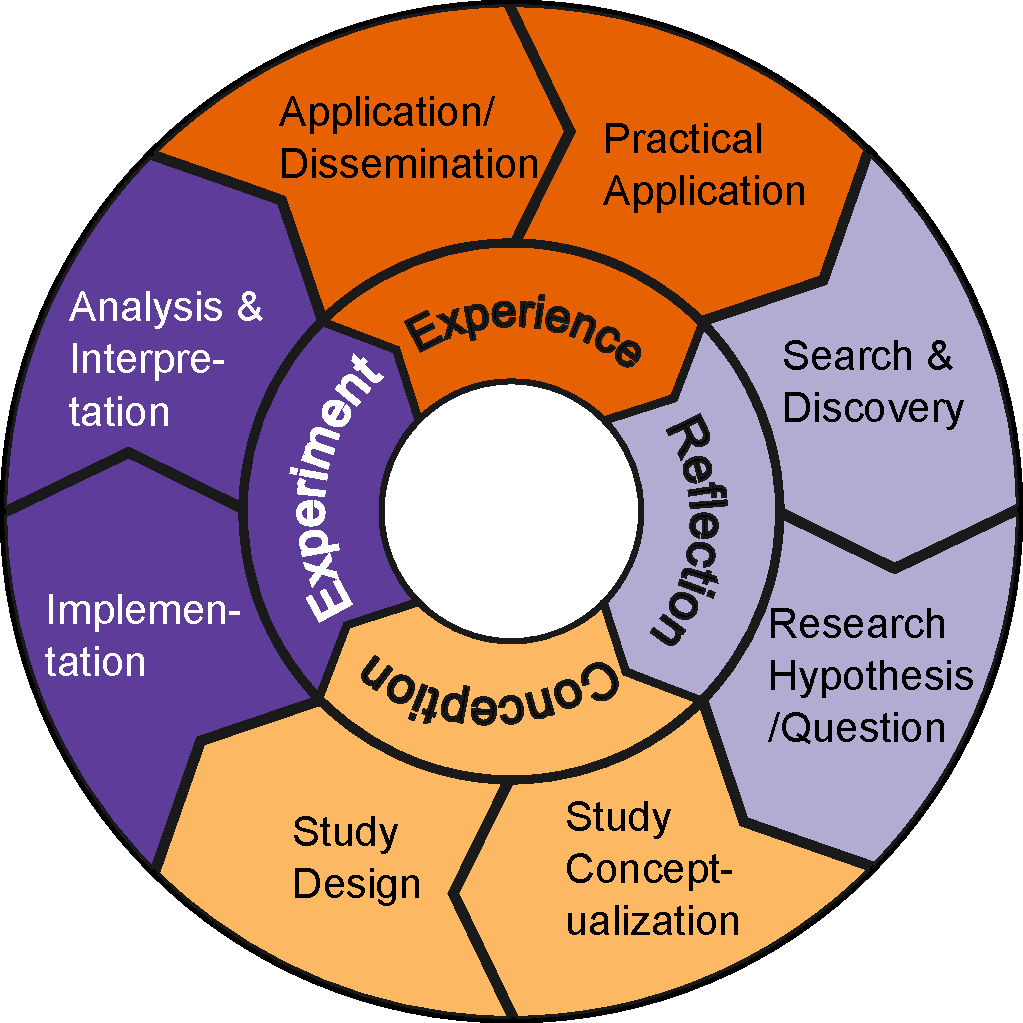
\includegraphics[width=0.7\linewidth,height=\textheight,keepaspectratio]{img/Research_cycle.pdf}

    }

    \caption{\label{fig-research_cycle}The research cycle based on
    \autocite{wildt2009forschendes} integrates the typical research
    process with the learning process.}

    \end{figure}%

    In the second example a GPT-like attention model is trained to
    classify data gained from the James-Webb telescope. Due to vast
    amounts of data and the continuous stream of new data research
    software engineering is needed to implement a pipeline for data
    cleaning, data warehousing and in-time analysis. In this case, the
    analysis \& interpretation phase (4) has much more relevance.
    Another point of this is example is that data science competencies
    such as vectorization of algorithms, statistical analysis, machine
    learning etc. are interconnected with competencies from software
    engineering such as software architectures, software project
    management, and database programming. In this case the distinction
    between DS competencies and RSE competencies is very fluid.

    The main argument behind these examples is that data science and
    research software engineering have a lot in common in terms of
    software development for science but show major differences where
    they are placed in the research process. This reframes the questions
    like ``how much programming is in DS'' or ``how much engineering is
    in RSE'' to a more structured approach of which cross-cutting
    functions exist in the research cycle that require computational
    means and which functions are part of the core identity of data
    scientists or research software engineers.

    As a working hypothesis based on the example above and experience in
    the field we assume the following: {[}H1{]} RSE focuses more on
    concept development (if the research is computationally heavy),
    design, implementation and dissemination, i.e.~phases 1,2,3,6
    whereas DS focuses more on analysis, interpretation and
    dissemination (phases 4,5,6). Moreover, a second hypothesis would be
    that RSE often plays a role in shaping the context of the research
    {[}H2a{]}, such as integrating projects with similar concerns, open
    source development and institutional needs. In contrast, data
    science is exclusively embedded in the research {[}H2b{]}.

    The focal point of the following chapter will revisit existing ideas
    for DS and RSE curricula and map the competences outlined there to
    the phases in the research process. This should give the abstract
    discussion above empirical grounding and can be used to test the
    hypothesis.

    \section{Comparison Method}\label{comparison-method}

    In the following the contents of \autocite{GI2021DataScience} is
    parsed as the most current examples of data science curricula in the
    German research context. The contents are inspected for obvious
    links to the research process and interpreted if no explicit
    connections are made. Further sources for data science curriculum is
    the output of the Edison Project \autocite{EDSF2017} and the
    OpenDS4all Project \autocite{OpenDS4All2020}.

    For the RSE side the contents of \autocite{Goth2024RSE} are used as
    a basis as well as the current state of the RSE-Curriculums project
    \autocite{RSECurriculums2021}. For the RSE competencies the RSE
    community has developed short codes. These are attached in the
    glossary in the attached repository \autocite{ds2rse2025}.

    In addition, relevant competences from the research data management
    field \autocite{petersen_2025_15025246} are included as they
    intersect with both DS and RSE.

    In terms of methodology it should be noted that this approach
    follows a community-driven consensus building. It should not be
    mistaken for a review study with measurable intersubjectivity based
    on instruments like PRISMA \autocite{Page2021PRISMA}.

    The lists of extracted DS and RSE competency clusters can be found
    in \autocite{ds2rse2025}. We also plan to publish a full table of
    RSE competencies (and possible DS competencies) sorted by clusters.
    In terms of this top-level discussion the competency clusters are
    sufficient to compare the differences with regard to the research
    cycle.

    \section{Discussion}\label{discussion}

    H1 could not be confirmed in the strict sense. Although the compiled
    competency clusters show that there is a stronger focus on certain
    stages of the research process for both RSE and DS competencies,
    both can be interpreted more generally to encompass all stages of
    the research cycle. Moreover, there are some competency description
    that seem very similar such as the focus on the research cycle for
    RSE and the data science lifecycle for DS. In terms of methodology
    simply comparing the existing mentions of competencies should not be
    regarded as the best possible proxy to the actual distribution in
    the field. A survey study asking practitioners and researchers where
    in the process they would place DS and RSE would yield far more
    convincing results. Still, self-evaluation might also be biased
    depending on the identity of the people working the in the
    respective fields.

    \begin{figure}[h!]
    \centering
    \begin{minipage}{0.48\textwidth}
    \centering
    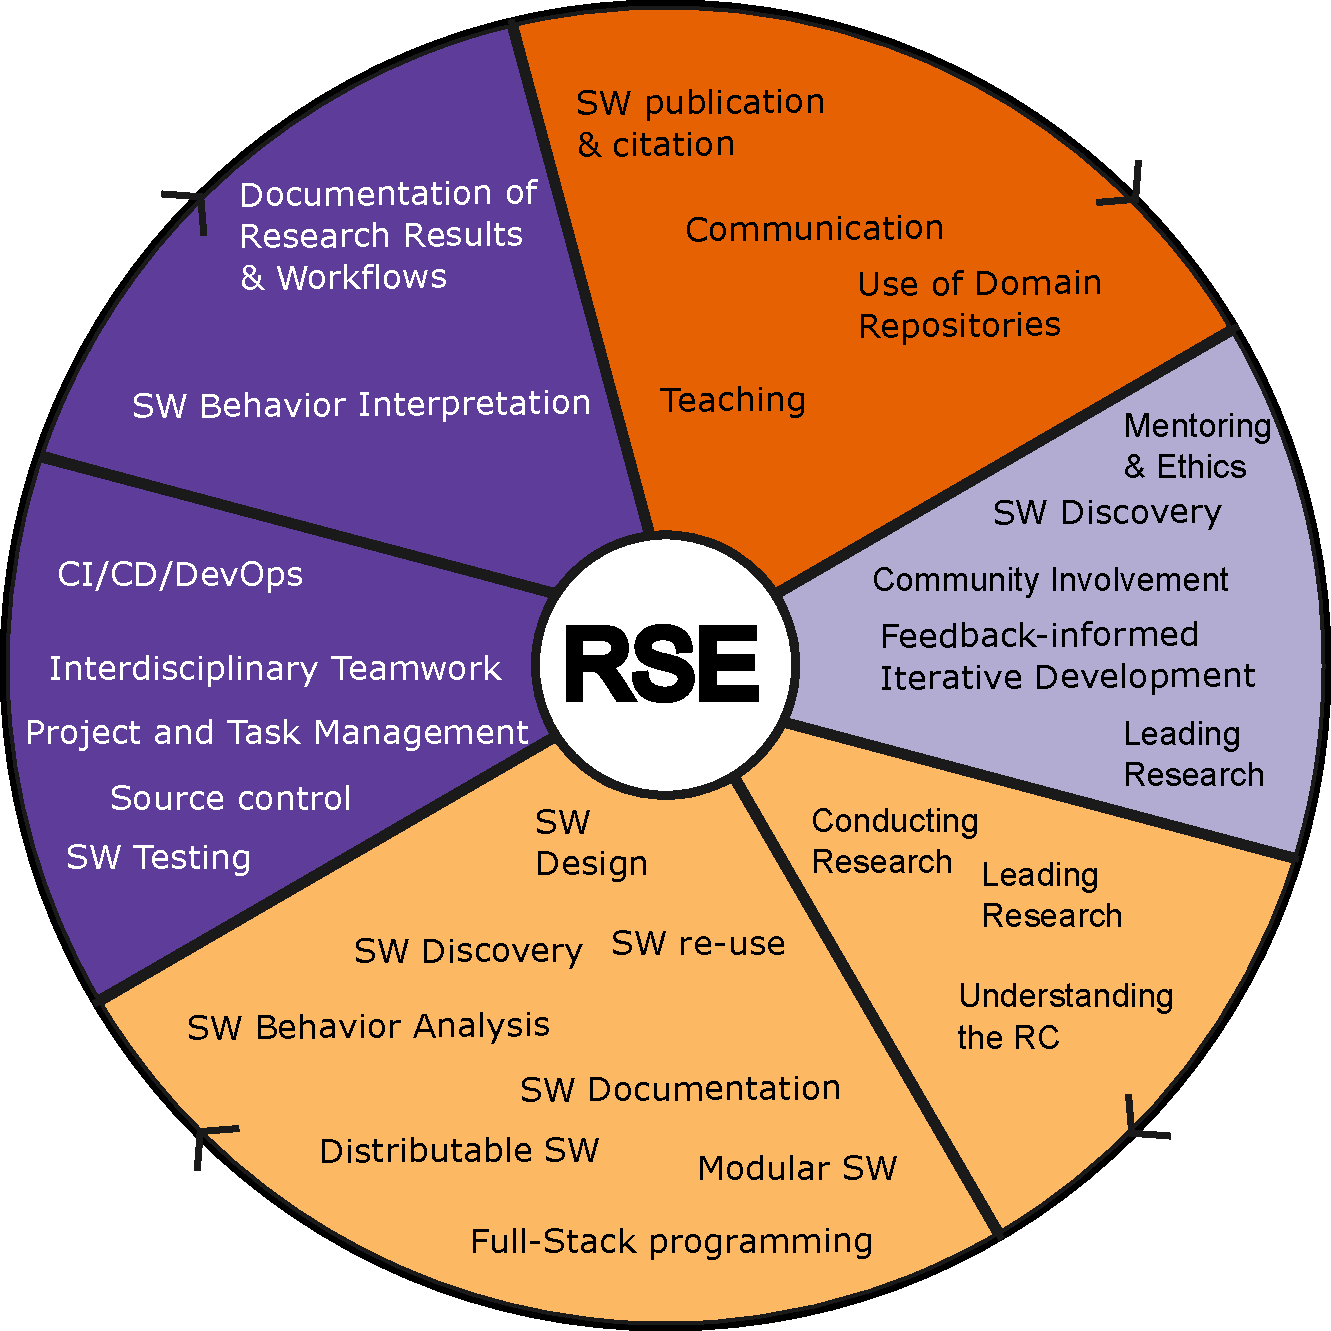
\includegraphics[width=\linewidth]{img/RC_RSE_competences.pdf}
    \caption{RSE Competences in the Research Cycle}
    \label{fig:rc_rse}
    \end{minipage}\hfill
    \begin{minipage}{0.48\textwidth}
    \centering
    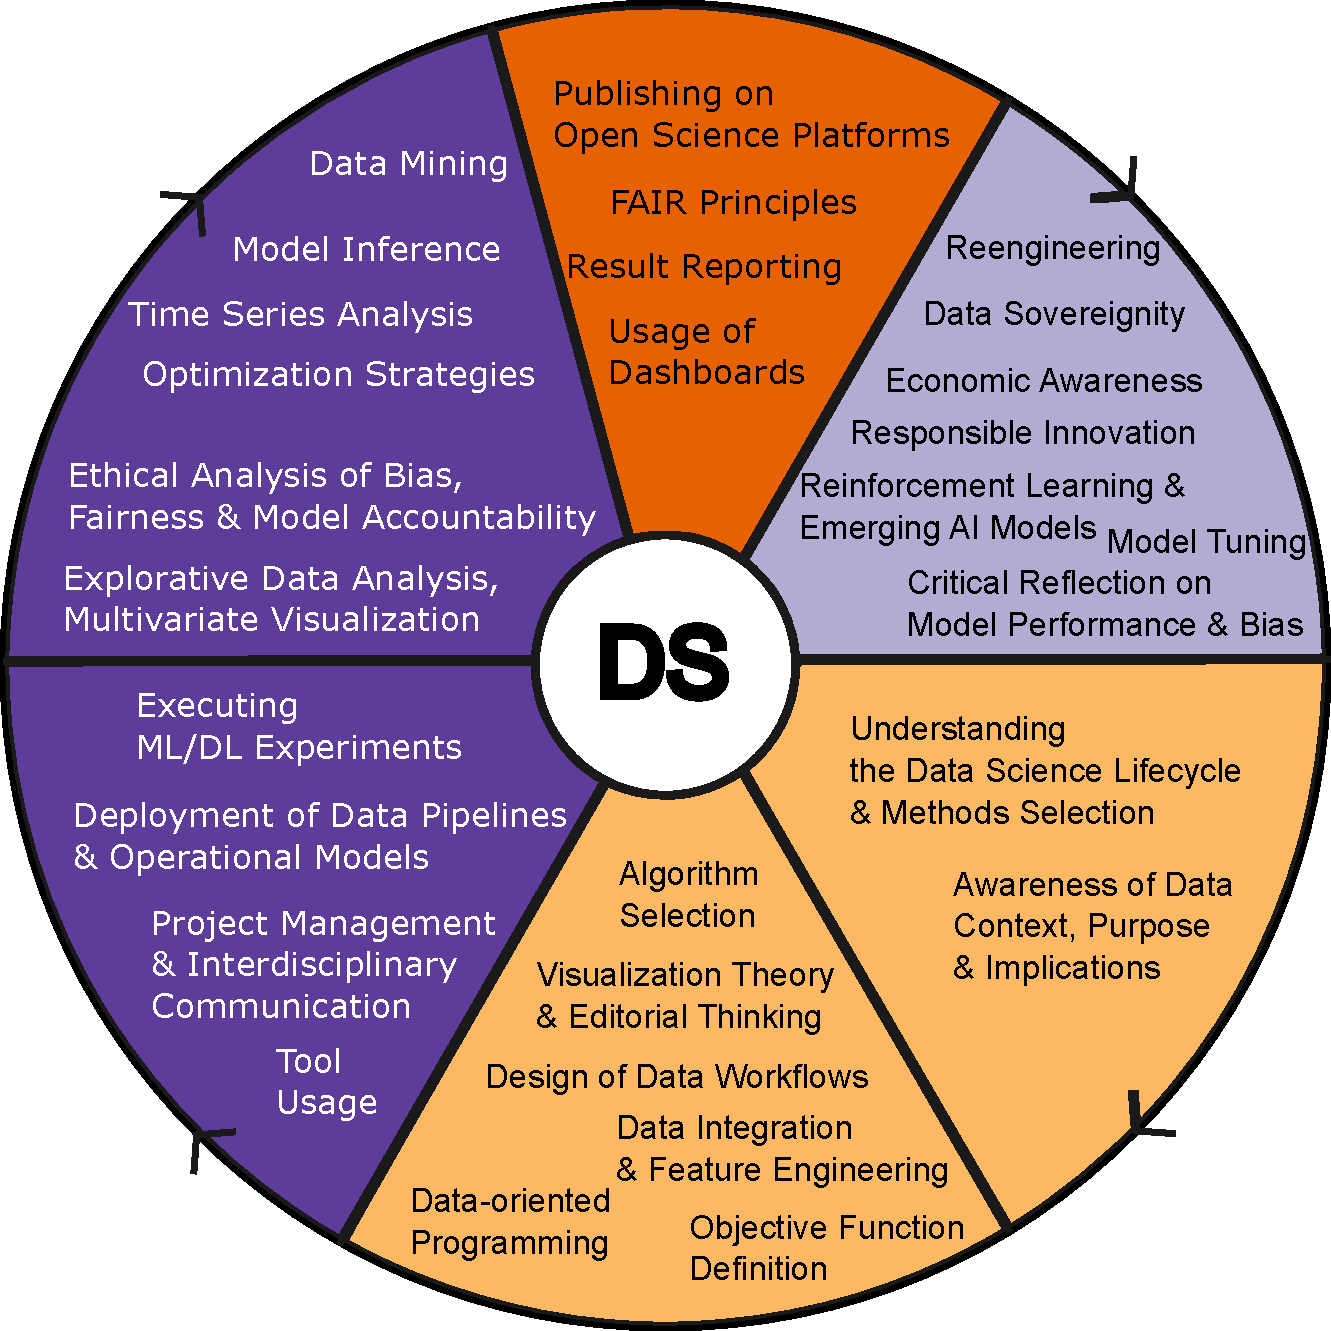
\includegraphics[width=\linewidth]{img/RC_DS_competences.pdf}
    \caption{DS Competences in the Research Cycle}
    \label{fig:rc_ds}
    \end{minipage}
    \end{figure}

    The most clear differences between DS and RSE are found in the
    design stage and the analysis stage. The design stage holds most of
    the competency clusters the RSE community defined. The DS
    counterpart is very general and many competencies listed there could
    in fact be construed as RSE-competencies that are imported for more
    complex cases. In contrast, the analysis stage is more connected to
    DS. This can be explained by the historic challenges software
    development faces in terms of clear-cut evaluation but also by the
    distribution of labor: if the RSE-job ends with the developed
    software and the core experiment or study uses the software as a
    tool, the analysis part is then handed over to the respective field
    specialists.

    Another reason for the design focus of RSE is the limited resources
    available. It is very time-consuming to both evaluate the impact of
    technology and also to evaluate the technology itself and its impact
    on the study. Comprehensive methods like Directed Acyclic Graph
    Modellings (DAGs) or Instrumental Variables try to tackle these
    nested evaluation issues but have not found widespread use. For that
    reason, the evaluation often concludes with the evaluation of the
    design part with instruments like the Technology Acceptance Model
    (TAM) or usability scales.

    H2 also had to be rejected: in fact, DS seems to contain more
    aspects outside the research cycle than RSE. Even though the core
    analysis of data component is very embedded in research, DS has a
    lot of institutional, political and legal challenges. Research Data
    Management (RDM) could be named as the most prominent of these. Due
    to the strong overlap of non-research related competencies, a joint
    list competency clusters was compiled that lists the competences
    that are not research cycle related (also in the repository
    \autocite{ds2rse2025}).

    The long list of transversal competencies begs the question if there
    are also technical competences that overlap. Even though this was
    not the focus of the analysis, these can be easily spotted by
    investigating the shift of data analysis to artificial intelligence
    based methods. Training, fine-tuning and mainstreaming large
    language models requires more and more computing power, stable
    infrastructure and network components. On the other hand, CPU-based
    software-engineering becomes less demanding and also profits from
    AI-generated algorithm and code development. However, not all
    software engineering boils down to the current AI-hype. In summary,
    there is no clear way of generalizing whether DS or RSE need more
    and deeper understanding of computer science.

    \section{Conclusion}\label{conclusion}

    We have given a short and non-exhaustive introduction into the
    profiles of the Research Data Manager, the Data Scientist, the
    Research Software Engineer, and the Research Infrastructure
    Engineers. The research cycle has served us as a useful reference on
    which to compare data science and research software engineering.
    While we found differences we have also seen commonalities. We hope
    that future work delineates the differences better in order to
    sharpen the profile. Also it will be beneficial for the curriculum
    development of both fields to understand their commonalities in
    order to share academic resources. We hope that this contribution
    can serve as an entry for more discussion about RSE in the Data
    Science community, and about the Data Science profile in the RSE
    community and thereby raising the awarenes about each other in the
    communities. Among the broader trends in our world, we expect that a
    collaboration between the communities can be beneficial to harness
    the AI trend in a manner that is beneficial for public science.

    \printbibliography

% Bibliography



\end{document}
